\section{Entity-relationship diagram}
An entity-relationship diagram (ER diagram) can express the structure of a database graphically \cite{DBConcepts}.
It serves as a way to gain a better understanding of the requirements of the database and to ensure its design is clear.
An ER diagram shows entity sets of the database and their relationships.
An entity is usually an object in the real world that is distinguishable from other objects, and is described through a set of attributes that make up an entry set.
Relationships are associations between entities.
Cardinalities are important for these relationships, as they express the number of entities to which another entity can be associated \cite{DBConcepts}, either one or many.
With these two cardinalities, the following mappings can be used:
\begin{itemize}
    \item One-to-one
    \item One-to-many
    \item Many-to-many
\end{itemize}
A one-to-one relationship means that an entity in an entity set A is associated with at most one entity in an entity set B, and an entity in B is associated with at most one entity in A.
A one-to-many relationship means that an entity in A is associated with any number of entities in B, and an entity in B can be associated with at most one entity in A.
For many-to-many relationships, an entity in A is associated with any number of entities in B, and an entity in B is associated with any number of entities in A \cite{DBConcepts}.
\autoref{fig:er-diagram} illustrates the physical design of the database for this system:
\begin{sidewaysfigure}[]
    \centering
    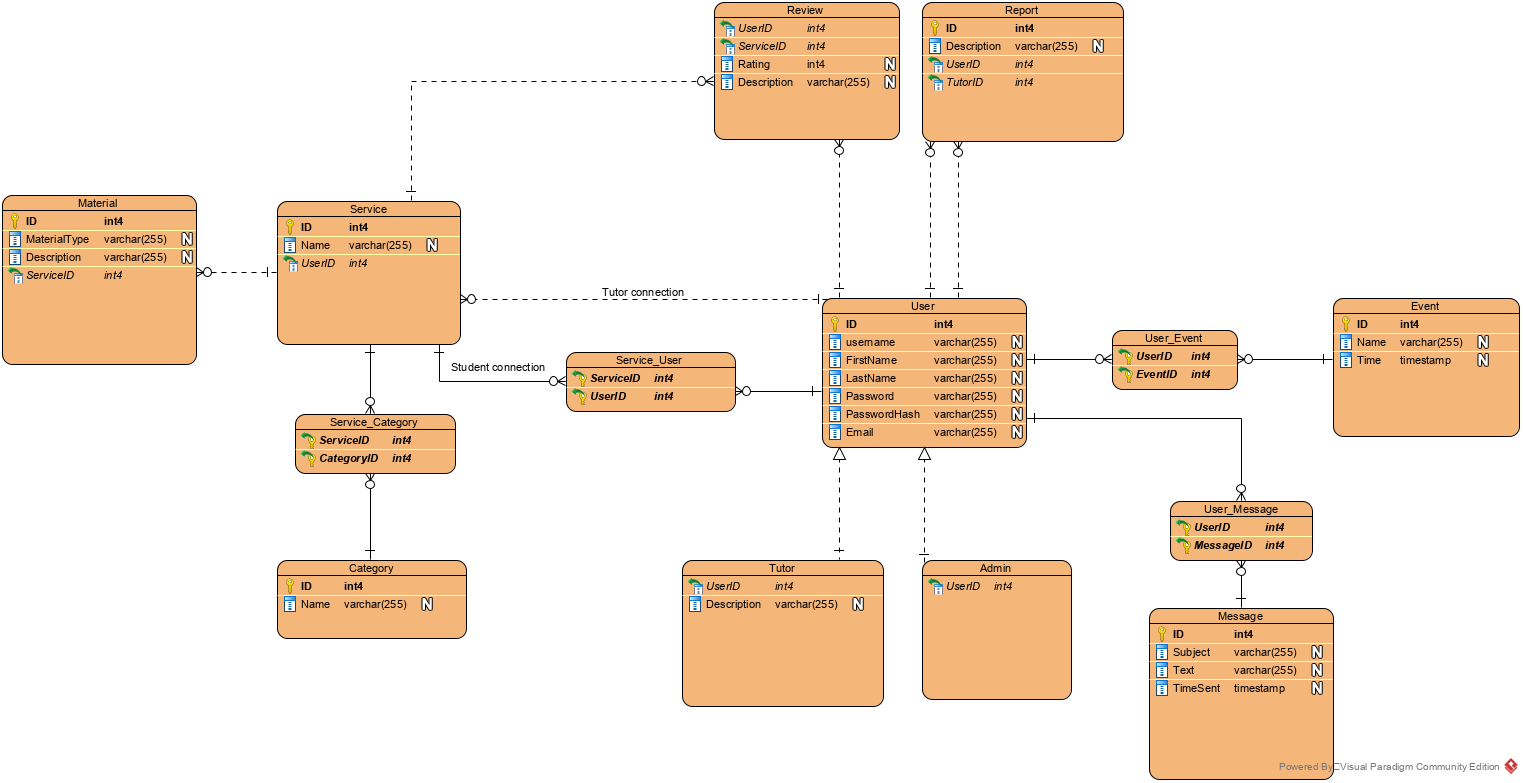
\includegraphics[width=\linewidth]{/s7erd.png}
    \caption{The ER diagram that illustrates the design of the database.}
    \label{fig:er-diagram}
\end{sidewaysfigure}
\\\\
In \autoref{fig:er-diagram}, entities are represented by the rectangular boxes.
The name of the entity set is in the header of the box, and the list of attributes is below the name, along with the type of each particular attribute.
\textit{User} is an example of an entity set.
Each entity is defined through the list of attributes shown below the name, such as \textit{ID}, \textit{Username} and \textit{FirstName}.
Relationships are represented by the lines between entities.
The way the line representing the relationship connects to the entity shows the cardinality of that relationship.
If the line ending is connected to the entity by the circle triangle combination, such as both connections to review, it means this side of the relationship has a cardinality of many.
If the line simply ends with another line crossing it such as the ones connected to tutor or admin, it has the cardinality of one.
\\\\
Starting from the left are the \textit{material} and \textit{service} entity sets connected through a relation.
A material entity has a number of attributes, such as a description of the material, a type such as article, text or video, and a unique identifier known as the primary key.
This primary key is the attribute \textit{ID}.
When an attribute is unique, it can be used to identify a given instance of the entity.
However, because of the one-to-many relationship between service and material, material also contains what is known as a foreign key in the attribute \textit{ServiceID}.
This foreign key references the primary key of the entity set that participates as the one side.
This ensures that for any entity in set \textit{material} you can use the foreign key to get the corresponding service.
\\\\
The relationship between \textit{service} and \textit{category} is a many-to-many relationship.
To model this, a separate entity set is created.
This entity set is named after the two participating sets, and has both primary keys as its attributes.
This ensures that for a particular entity in the set \textit{service}, it can be related to multiple entities of the set \textit{category}.
In the database, this would be achieved through multiple entities of the \textit{service\_category} being present with the same \textit{ServiceID} attributes, but each instance is linked to a different \textit{CategoryID} attribute.
Another example of a many-to-many relation is users and messages, where a message is associated with a sender, and at least one receiver.
\\\\
A particularly interesting entity set is the \textit{user} set.
As defined in the \autoref{fig:class-diagram}, the admin and tutor properties are viewed as specializations through roles.
This is achieved in the ER diagram by modeling them as subtypes, defining an \textit{ISA} relationship, which is represented by the arrow from both \textit{tutor} and \textit{admin}.
They show that a tutor is a user, and in the same way, an admin is a user.
However, for the physical design, this would be achieved through separate tables for both tutors and admins, in which the attributes specific to those roles are defined along with a key that links it together with a user from the user table to get those attributes as well.
The user entity set has multiple connections to another entity set - \textit{report}.
The reason for this is due to the subtypes.
As a user can be both a student and a tutor, this needs to be reflected in the relationship.
A report is made by a student targeting a tutor.
As such, we model it through two relations to the user entity set, in order to get a foreign key for both the reporting student and the tutor being reported.
